\documentclass[10pt]{article}
\usepackage{amsmath,textcomp,amssymb,geometry,graphicx,enumerate,tikz,algorithm,algpseudocode,pifont}
\usetikzlibrary{calc}
\usetikzlibrary{datavisualization}
\usetikzlibrary{datavisualization.formats.functions}


\textheight=9in
\textwidth=7in
\topmargin=-.75in
\oddsidemargin=-0.25in
\evensidemargin=-0.25in

\usepackage{listings}
\lstnewenvironment{codeblock}
    {\lstset{language=Python,
      showspaces=false,
      showtabs=false,
      breaklines=true,
      mathescape=true,
      showstringspaces=false,
      breakatwhitespace=true,
      commentstyle=\textit,
      keywordstyle=\textbf,
      basicstyle=\ttfamily,
      escapechar=`,
      moredelim={**[is][{\color{RoyalBlue}}]{\^^M\\beginsol}{\^^M\\endsol}},
      moredelim={[is][{\color{RoyalBlue}}]{\^^M\\beginexp}{\^^M\\endexp}},
    }}
    {}
    
\begin{document}
\section*{01/25/2016}
\subsection*{Classifiers}
		\ 
		\begin{itemize}
			\item You are given a set of n \underline{samples}, each with d features.

			\item Some samples belong to a certain \underline{class} $\mathcal{O}$; some do not.

			\item Example: sample are bank loans, features are income and age (d=2). Some are in class defaulted; some are not. \underline{Goal}: Predict whether future borrowers will default based on their income and age.

			\item Represent each sample as a point in a d-dimensional space, called a \underline{feature vector} (aka predictors, independent variables).

			\item \underline{Decision boundary}: the boundary chosen by our classifier to separate $\mathcal{O}$ from not $\mathcal{O}$.

			\item Some (not all) classifiers work by computing a \underline{predictor function}: A function $f(x)$ that maps sample point $x$ to a scalar such that,
				\begin{align*}
					& f(x) > 0 \ if \ x \ \in class \ \mathcal{O} \\
					& f(x) \leq 0 \ if \ x \ \notin \ class \ \mathcal{O}\\
				\end{align*}
				(aka decision function, or discriminant function).
				
			\item For these classifiers, the decision boundary is, 
				$$ \{x \in \mathbb{R}^{d}: f(x) = 0 \} $$
				That is the set of all points where the prediction function is zero. Usually this set is a ($d-1$)-dimensional surface in $\mathbb{R}^{d}$.

			\item $\{ x: f(x) = 0 \}$ is also called an \underline{isosurface} (aka isocontours) of $f$ for the \underline{isovalue} 0.

			\item \underline{Linear classifier}: The decision boundary is a hyperplane. Usually uses a linear predictor function.

			\item \underline{Overfitting}: when sinuous (having many curves and turns) decision boundary fits sample data so well that it doesn't classify future (test set) items well.
		\end{itemize}
		
%%%%%%%%%%%%%%%%%%%%%%%%%%%%%%
	\subsection*{Math Review}
		\
		\begin{itemize}
			\item \underline{Vectors}:
			$$
				x = \begin{bmatrix}
 					x_{1} \\
 					x_{2} \\
 					x_{3} \\
 					x_{4} \\
 					x_{5} 
 				\end{bmatrix}
 				= \begin{bmatrix}
 					x_{1} & x_{2} & x_{3} & x_{4} & x_{5}
 				\end{bmatrix}^{T}
			$$
			Think of $x$ as a point in $\mathbb{R}^{d}$.
			
			\item Conventions (often, but not always):
				\begin{itemize}
					\item Uppercase roman = matrix.
					\item Lowercase roman = vector.
					\item Greek = scalar.
					\item Other scalars: n = number of samples, d = number of features or dimension of sample, i, j, and k = indices.
					\item Functions (often scalars): $f()$, $s()$, etc.
				\end{itemize}
			\item \underline{Inner products} (aka dot products)
				\begin{itemize}
					\item $x \cdot y = x_{1}y_{1} + x_{2}y_{2} + \dots + x_{d}y_{d}$
					\item Also written $x^{T}y$.
					\item Clearly, $f(x) = w \cdot x + \alpha$ is a linear function in $x$.
				\end{itemize}
			\item \underline{Eucledian norms}: $||x|| = \sqrt{x \cdot x} = \sqrt{x_{1}^{2} + {x_{2}^{2} + \dots + x_{d}^{2}}}$
				\begin{itemize}
					\item $||x||$ is the length (aka Eucledian length) of a vector $x$.
					\item Given a vector $x$, $\frac{x}{||x||}$ is a unit vector (length 1).
					\item "Normalize" a vector $x$: replace $x$ with  $\frac{x}{||x||}$.
				\end{itemize}
			\item Use dot product to compute angles:\\
				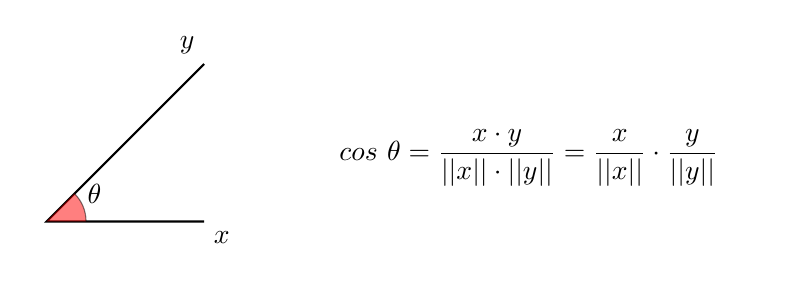
\begin{tikzpicture}
					\coordinate[label=below left:$$] (A) at (0,0);
					\coordinate[label=below right:$x$] (X) at (2,0);
					\coordinate[label=above left:$y$] (Y) at (2,2);

					\draw[thick] (X) -- (A) -- (Y);

					% Mark the angle XAY
					\begin{scope}
					\path[clip] (A) -- (X) -- (Y);
					\fill[red, opacity=0.5, draw=black] (A) circle (5mm);
					\node at ($(A)+(30:7mm)$) {$\theta$};	
					\end{scope}
				\node[text width=6cm, anchor=west, right] at (3,1)
    			{$$cos \ \theta = \frac{x \cdot y}{||x|| \cdot ||y||} = \frac{x}{||x||} \cdot \frac{y}{||y||}$$};
    			\end{tikzpicture}
    			
    			\begin{tikzpicture}
					\coordinate[label=below left:$$] (A) at (0,0);
					\coordinate[label=below right:$$] (X) at (2,0);
					\coordinate[label=above left:$$] (Y) at (2,2);

					\draw[thick] (X) -- (A) -- (Y);

					% Mark the angle XAY
					\begin{scope}
					\path[clip] (A) -- (X) -- (Y);
					\fill[red, opacity=0.5, draw=black] (A) circle (5mm);
					\node at ($(A)+(30:7mm)$) {$\theta$};	
					\end{scope}
				\node[text width=6cm, anchor=west, right] at (3,1)
    			{$$acute, \ cos \ \theta > 0$$};
    			\end{tikzpicture}

    			\begin{tikzpicture}
					\coordinate[label=below left:$$] (A) at (0,0);
					\coordinate[label=below right:$$] (X) at (2,0);
					\coordinate[label=above left:$$] (Y) at (0,2);

					\draw[thick] (X) -- (A) -- (Y);

					% Mark the angle XAY
					\begin{scope}
					\path[clip] (A) -- (X) -- (Y);
					\fill[red, opacity=0.5, draw=black] (A) circle (5mm);
					\node at ($(A)+(30:7mm)$) {$\theta$};	
					\end{scope}
				\node[text width=6cm, anchor=west, right] at (3,1)
    			{$$right, \ cos \ \theta = 0$$};
    			\end{tikzpicture}
    			
    			\begin{tikzpicture}
					\coordinate[label=below left:$$] (A) at (1,0);
					\coordinate[label=below right:$$] (X) at (3,0);
					\coordinate[label=above left:$$] (Y) at (0,2);

					\draw[thick] (X) -- (A) -- (Y);

					% Mark the angle XAY
					\begin{scope}
					\path[clip] (A) -- (X) -- (Y);
					\fill[red, opacity=0.5, draw=black] (A) circle (5mm);
					\node at ($(A)+(30:7mm)$) {$\theta$};	
					\end{scope}
				\node[text width=6cm, anchor=west, right] at (3,1)
    			{$$obtuse, \ cos \ \theta < 0$$};
    			\end{tikzpicture}
    		
    		\item Given a linear predictor function $f(x) = w \cdot x + \alpha$, decision boundary is
				$$ H = \{ x : w \cdot x = - \alpha \} $$
				\begin{itemize}
					\item The set $H$ is called a hyperplane (A line in 2D, a plane in 3D).
				\end{itemize}
				
			\item \underline{Theorem}: Let $\vec{xy}$ be a vector that lies in $H$. Then $w \cdot (y - x) = 0$. \\
				\underline{Proof}: $x$ and $y$ lie on the hyperplane H. $\therefore w \cdot (y - x) = -\alpha - (-\alpha) = 0$.
				
			\item $w$ is called the \underline{normal vector} of $H$. $w$ is normal (perpendicular) or orthogonal to $H$.

			\item If $w$ is a unit vector, $w \cdot x + \alpha$ is called the \underline{signed distance} from $x$ to $H$ i.e. its distance, but positive on one side of $H$; negative on the other. Moreover the distance from $H$ to the origin is $\alpha$. Hence $\alpha = 0$ if and only if $H$ contains the origin.
			
			\item The coefficients in $w$, plus $\alpha$ are called \underline{weights} or \underline{regression coefficients}. Goal of many Machine Learning algorithms is to find what the weights should be.
			
			\item The input data is linearly separable if $\exists$ a hyperplane that separates all samples $\in \mathcal{O}$ from all samples $\notin \mathcal{O}$.
			\end{itemize}

%%%%%%%%%%%%%%%%%%%%%%%%%%%%%%%%
	\subsection*{Perceptron algorithm}
		\
		\begin{itemize}
			\item (Frank Rosenblatt, 1957) Slow, but correct for linearly separable samples. Uses a \underline{numerical optimization} algorithm: \underline{gradient descent}.
			
			\item Consider $n$ sample vectors $x_{1}, x_{2}, \dots x_{n}$.
			
			\item For each sample, let
				\[
 					y_{i} = \left\{\def\arraystretch{1.2}%
 						\begin{array}{@{}c@{\quad}l@{}}
    						1 & \text{if $x_{i} \in \mathcal{O}$}\\
    						-1 & \text{if $x_{i} \notin \mathcal{O}$}\\
  						\end{array}\right.
				\]
			
			\item Goal: find weights $w$ such that
				\begin{align*}
					& x_{i} \cdot w \geq 0 \ \ \ \text{if} \ y_{i} = 1 \\
					& x_{i} \cdot w \leq 0 \ \ \ \text{if} \ y_{i} = -1\\
				\end{align*}
			 
			 \item Equivalently: $y_{i}x_{i} \cdot w \geq 0$. Inequality is called a \underline{constraint}.
			 
			 \item Idea: We define a \underline{risk function} $R$ that is positive if some constraint is violated. Then we use optimization to choose $w$ that minimizes $R$.
			 
			 \item Define the \underline{loss function}
			 	\[
 					L(y, y_{i}) = \left\{\def\arraystretch{1.2}%
 						\begin{array}{@{}c@{\quad}l@{}}
    						0 & \text{if $y_{i}y \geq 0 $}\\
    						-y_{i}y & \text{otherwise}\\
  						\end{array}\right.
				\]
			
			\item Define the \underline{risk function} (aka \underline{objective function} or \underline{cost function})
				$$ R(w) = \sum_{i=1}^{n} L(x_{i} \cdot w, y_{i}) = 
					\sum_{i \in V} -y_{i} \cdot x_{i} \cdot w $$
				where $x_{i} \cdot w$ is our prediction, $y_{i}$ is the correct classification and $v$ is the set of indices $i$ for which $y_{i}x_{i} \cdot w < 0$.
			\item If $w$ classifies $X_{1}, \dots, X_{n}$ correctly, then $R(w) = 0$. Otherwise, $R(w) > 0$; we want to find a better $w$.
			
			\item \textbf{\underline{Goal}: Solve this \underline{optimization problem}; Find $w$ that minimizes $R(w)$.}
	\end{itemize}
\end{document}